\chapter{Experiments}\label{chapter:experiments_and_results}
As mentioned in the previous chapter, the process of finding was an iterative one of running an experiment, analyzing the generated data, draw conclusions and then repeat the steps with a new experiments designed to amend the mistakes of the previous experiment. This chapter will go through the results that were obtained from each of the data sets. A summary and discussion of the results is found in chapter \ref{chapter:discussion}.

\section{Overview of experiments}
The model has many parameters, and doing an exhaustive search over the entire parameter space is not possible. Instead, a genetic algorithm (GA) was used to do targeted searches of the parameters. For the details of the GA, please see chapter \ref{chapter:ga}. Depending on how the GA was set up, different areas of the search space was searched. Even when using a GA, some parameters had to be fixed. However, fixing parameters means that the effect of the fixed parameter on the behavior of the model remains unknown, since only a subspace of the entire parameter space is searched. For this reason the genetic algorithm was executed several times, each creating a data set containing fitness values for different parts of the parameter space. Each of these data set can be analyzed, providing information which can be corroborated in order to form an understanding of the overall market behavior.

Table \ref{table:datasets_overview} contains an overview of the different data sets, showing which parameters were fixed, and which were included as genes in the genetic algorithm.

In the following four experiments, the genetic algorithm was set to minimize all four fitness-measures.

\begin{description}
\item[\dthree: Varying the number of HFT agents, and all latency related parameters] This data set was generated by including all the model parameters concerning time latency as well as the number of agents into the individuals in the genetic algorithm. Due to the high number of variables, the data turned out to be difficult to analyze, as too many factors pertaining to the simultaneous change of several parameters influenced the fitness values.
\item[\dnine: Fixing the number of agents while varying latency parameters] The analysis of \dthree{} showed that when minimizing the four fitness-measures, the genetic algorithm tended to select  model containing few or no HFT agents. The case of a market with no market makers and no chartists can safely be said to be trivial. Hence, in experiment \dnine, the number of HFT agents were fixed to $\ssmmnAgents = 30$ and $\scnAgents = 100$.
\item[\dten: Fixing the number of HFT chartists] Since \dnine kept \ssmmnAgents and \scnAgents constant, the experiment did not reveal anything on how the market behavior changes when the number of agents changes. In order to investigate the impact of having many or few HFT market makers, \ssmmnAgents was varied in this experiment. Although it is also of interest how the market behavior depends on the number of HFT chartists, including \scnAgents as a gene would yield results similar to those obtained in \dthree. For this reason the number of HFT chartists was fixed to $\scnAgents = 150$.
\item[\deleven: Fixing the number of HFT market makers] This experiment was carried out in order to investigate the impact of the number of HFT chartists on the market behavior, and is supplementary to \dten.
\end{description}


\begin{table}
\begin{tabular}{|l|L|E|L|}
\toprule
ID & Description & Fixed parameters& As genes \\
\midrule
\dthree & All parameters varied& $\scordervolumemu=10$,$\scordervolumes=3$,$\ssmmordervolumemu=50$,$\ssmmordervolumes=20$,$\scticksbeforereactingmu=2$,$\scticksbeforereactings=5$,$\scpriceticksizemu=3$,$\scpriceticksizes=2$ &  \sclatencymu, \sclatencys, \scnAgents, \scthinkmu, \scthinks, \sctimehorizonmu, \sctimehorizons, \scwaitTimeBetweenTradingmu, \scwaitTimeBetweenTradings, \ssmmlatencymu, \ssmmlatencys, \ssmmnAgents, \ssmmthinkmu, \ssmmthinks\\
\midrule
\dnine & Fixed number of HFT agents &$\ssmmnAgents = 30$, $\scnAgents = 100$,$\scordervolumemu=10$,$\scordervolumes=3$,$\ssmmordervolumemu=50$,$\ssmmordervolumes=20$,$\scticksbeforereactingmu=2$,$\scticksbeforereactings=5$,$\scpriceticksizemu=3$, $\scpriceticksizes=2$ & \scthinkmu, \scthinks, \sctimehorizonmu, \sctimehorizons, \scwaitTimeBetweenTradingmu, \scwaitTimeBetweenTradings, \ssmmlatencymu, \ssmmlatencys, \ssmmnAgents, \ssmmthinkmu, \ssmmthinks \\
\midrule
\dten & Fixed number of HFT chartists and fixed strategy parameters & $\scnAgents = 150$, $\ssmmthinkmu = \scthinkmu = 50$, $\ssmmthinks = \scthinks = 20$, $\sctimehorizonmu = 5000$, $\sctimehorizons = 2000$, $\scwaitTimeBetweenTradingmu = 50$, $\scwaitTimeBetweenTradings = 20$,$\scordervolumemu=10$,$\scordervolumes=3$,$\ssmmordervolumemu=50$,$\ssmmordervolumes=20$,$\scticksbeforereactingmu=2$,$\scticksbeforereactings=5$, $\scpriceticksizemu=3$,$\scpriceticksizes=2$  & \ssmmnAgents, \sclatencymu, \sclatencys, \ssmmlatencymu, \ssmmlatencys \\
\midrule
\deleven & Fixed number of HFT market makers and fixed strategy parameters & $\ssmmnAgents = 52$, $\ssmmthinkmu = \scthinkmu = 50$, $\ssmmthinks = \scthinks = 20$, $\sctimehorizonmu = 5000$, $\sctimehorizons = 2000$, $\scwaitTimeBetweenTradingmu = 50$, $\scwaitTimeBetweenTradings = 20$,$\scordervolumemu=10$,$\scordervolumes=3$,$\ssmmordervolumemu=50$,$\ssmmordervolumes=20$,$\scticksbeforereactingmu=2$,$\scticksbeforereactings=5$, $\scpriceticksizemu=3$,$\scpriceticksizes=2$  & \ssmmnAgents, \sclatencymu, \sclatencys, \ssmmlatencymu, \ssmmlatencys \\
\bottomrule
\end{tabular}
\caption{Overview of datasets}
\label{table:datasets_overview}
\end{table}


\subsection{Correlation between fitness measures}\label{section:correlation_fitness}
A factor which influences the evolution of parameters is correlation between the fitness-measures. If two or more fitness measures have non-negative correlation coefficients, individuals will be statistically more likely to get good scores in the correlated fitness measures at the same time. Since all fitness measures are given equal weight in the selection process, individuals scoring well in the correlated fitness-measures will win over individuals which score well on another, statistically independent fitness measure. It is therefore important to compare the selection tendencies with the correlation between fitness-measures. Figure \ref{figure:d10_fitness_correlation} shows a plot of the correlation matrix for \dten. Since later generations will be affected by the biased selection and therefore contain more individuals which did well on the correlated fitness measures, the correlation coefficients in the figure were calculated over individuals in the first generation only.
\begin{figure}
\centering

\includegraphics[width=0.7\textwidth]{Electron.pdf}
\caption{Correlation matrix of the four fitness measures in the first generation of dataset \dten	}
\label{figure:d10_fitness_correlation}
\end{figure}

For instance, the correlation between \overshoot and \stdev means that an individual which scores a good \overshoot-fitness will be statistically likely to also score a good \stdev-fitness. Since all four fitness measures are weighed evenly in the selection, models with behavior which is assigned good values for \overshoot and \stdev will score a better overall fitness than a simulation with a good fitness 

In other words, the correlation between \stdev and \overshoot means that stable individuals will outlive fast individuals as they are selected for breeding more often. This is not a property of a model itself, but rather a problem with the definition of the fitness measures. This problem can be circumvented by not using of the correlated fitness values. XXX

Both \overshoot and \stdev were used for the GA selection, and although these two fitness measures do reflect different properties of the simulations, they were found to be somewhat correlated. That is, a simulation which tends to have a small overshoot also tends to have stable traded prices. 

 (simulations with a small overshoot also tend to have more stable trade prices), and there work together towards selecting the same type of simulations. \timetoreachnewfundamental and \roundstable both  The same is not the case for \timetoreachnewfundamental and \roundstable, as it possible that a simulation responds quickly to the shock, but does not stay within the stability margin. 

\section{Fitness and parameter evolution}\label{section:fitness_and_paraeter_evolution}


\subsection{Variable number of market makers}

Figure \ref{fig:d10_evolution_fitness} shows the evolution of the four fitness measures. The population wide mean is plotted along the median and minimum statistics. Since all four fitness measures were minimized, the curve for the minimum value shows the best individual alive during each generation, with respect to each fitness measure. While the mean reflects how the overall population is evolving,  the median is useful as it gives an insight into how skewed the population wide distribution of parameters is. 


\begin{figure}
	%issue 15
	\centering
	\subcaptionbox{Evolution of \roundstable\label{fig:d10_evolution_fitness_a}}
	[0.49\linewidth]{\includegraphics[width=0.5\textwidth]{82_generation_plots/d10/round_stable.png}}
	\subcaptionbox{Evolution of \timetoreachnewfundamental\label{fig:d10_evolution_fitness_b}}
	[0.49\linewidth]{\includegraphics[width=0.5\textwidth]{82_generation_plots/d10/time_to_reach_new_fundamental.png}}
	\subcaptionbox{Evolution of \stdev\label{fig:d10_evolution_fitness_c}}
	[0.49\linewidth]{\includegraphics[width=0.5\textwidth]{82_generation_plots/d10/stdev.png}}
	\subcaptionbox{Evolution of \overshoot\label{fig:d10_evolution_fitness_d}}
	[0.49\linewidth]{\includegraphics[width=0.5\textwidth]{82_generation_plots/d10/overshoot.png}}
	\caption{Evolution of the four fitness measures in experiment \dten}
	\label{fig:d10_evolution_fitness}
\end{figure}





\begin{description}
\item[Model stability]
Figure \ref{fig:d10_evolution_fitness_a}: shows that  the GA quickly manages to find some parameters which cause the simulation to stabilize quickly. However, these individuals do not manage to dominate the population evident by the mean and median curves remaining almost the same until generation 30 or so. In the next 20 generations the population undergoes a rapid change, as the population wide average of \roundstable drop from close to $10^5$ to around $2\cdot 10^4$ rounds on average. The disparity between the mean and the median indicates that the population undergoes a rapid change in the same period, from mostly containing unstable individuals to mostly containing stable individuals. In generation 42, the median curve crosses the mean curve, which means that the the population contain as many stable simulations as it contain unstable simulations. From that point on the unstable simulations are quickly replaced by stable individuals.
\item[Price fluctuations and overshoot]
During the same period, the population average \stdev also decreases fairly rapidly, but the drop is less pronounced than the drop in \stdev. As figures \ref{fig:d10_evolution_parameters_a} and \ref{fig:d10_evolution_parameters_b} show, the number of market makers rapidly increased during this period, as did the average latency of the market makers. Since the mean and median are close in both figure\footnote{Since \overshoot is discrete, the median and $\min$ statistics are also discrete}, the mean is representative of the evolution of the entire population.
\item[Responsiveness]
\timetoreachnewfundamental measures the time it takes for the model to react to the shock in the fundamental, and the evolution of the population wide statistics is shown on figure \ref{fig:d10_evolution_fitness_b}. Although the GA is instructed to minimize \timetoreachnewfundamental in order to look for more faster models, it clearly fails to do this. Indeed, the most responsive simulation took only about 4000 rounds to reach the new fundamental, but this individual died out in favor of slower individuals. In the last generation the most responsive simulation took around 14000 rounds to reach the new fundamental. The reasons for this failure to locate responsive models is discussed in section \ref{section:correlation_fitness}. In the A large change of the average of \timetoreachnewfundamental happens in the rounds five to 15. In this period, the median is lower than the mean, which means that the growth in the mean can be attributed to a minority of individuals.
\end{description}


On figures \ref{fig:d10_evolution_fitness} and \ref{fig:d10_evolution_parameters}, the two areas shaded in a light blue and light red respectively show the two periods during which there was a drastic change in parameters and fitness-values. By comparing the time at which parameters and fitness-values change, it is possible to get an idea of how parameters influence the fitness-values. To that end, figure \ref{fig:d10_evolution_parameters} shows the evolution of each of the parameters that were varied by the GA\footnote{Since the median was found to follow the mean nicely for all the parameters, the medians are not displayed. Also, the gray error bars show the population wide variance}.
\begin{figure}
	%issue 15
	\centering
	\subcaptionbox{Evolution of \ssmmlatencymu{} and \sclatencymu\label{fig:d10_evolution_parameters_a}}
	[0.49\linewidth]{\includegraphics[width=0.5\textwidth]{82_generation_plots/d10/latpars_mu.png}}
	\subcaptionbox{Evolution of \ssmmlatencys{} and \sclatencys\label{fig:d10_evolution_parameters_b}}
	[0.49\linewidth]{\includegraphics[width=0.5\textwidth]{82_generation_plots/d10/latpars_s.png}}
	\subcaptionbox{Evolution of \ssmmnAgents\label{fig:d10_evolution_parameters_c}}
	[0.49\linewidth]{\includegraphics[width=0.5\textwidth]{82_generation_plots/d10/nAgents.png}}
	\caption{Evolution of the model parameters in experiment \dten}
	\label{fig:d10_evolution_parameters}
\end{figure}

The two periods indicated by the shaded squares seem to reflect some sudden changes in the parameters.

\begin{description}
\item[Average agent latency]  As is shown on figure \ref{fig:d10_evolution_parameters_a}, individuals containing large latency parameters are selected for both HFT market makers and HFT chartists. $\E{\sclatencymu}$ grows grows quickly during the first 20 rounds (blue shade). Referring back to figure \ref{fig:d10_evolution_fitness}, it is seen that $\E{\timetoreachnewfundamental}$ and $\E{\overshoot}$ grows and shrinks respectively. As for $\E{\ssmmlatencymu}$, it grows from rounds 20 through 50 (red shade), and this  seems to be strongly reflected in the growth of $\E{\roundstable}$, and to a lesser degree a decline in $\E{\overshoot}$ and $\E{\stdev}$. Furthermore, the small size of the error bars on both curves show that the population consistently moves towards containing more individuals with larger latency parameters for both HFT agent types. While initially $\E{\ssmmlatencymu} \approx \E{\sclatencymu}$, the population wide mean $\E{\sclatencymu}$ ends up being roughly 1.5 times larger than $\E{\sclatencymu}$. Finally, note also that the growth of  $\E{\sclatencymu}$ and $\E{\ssmmlatencymu}$ seem to be somewhat independent, as they sometimes grow together, sometimes not.

\item[Number of market makers] The number of market makers increases almost every generation, but grows especially quickly through rounds 20 to 50 (red shade)

\item[Agent latency variance] Figure \ref{fig:d10_evolution_parameters_b}: The trends for $\E{\sclatencys}$ and $\E{\ssmmlatencys}$ are less clear, as the population-wide variances $\Var{\sclatencymu}$ and $\ssmmlatencymu$ illustrated by the large error bars are high compared to the change in $\E{\sclatencymu}$ and $\E{\ssmmlatencymu}$. While this could mean that the simulation behaves more nicely when the difference between the latency parameters of the trading agents is smaller, further experiments would have to be carried out to confirm this fact. XXX
\end{description}

In summary, the genetic algorithm prefers simulations with many, but relatively slow market makers. Apparently simulations with slow chartists also outperformed those with fast chartists, but since the number of HFT chartists was fixed at $\scnAgents = $, this experiment does not reveal how the simulation would perform with more (or less) chartists. It is possible to imagine that the market would perform just as well with a few and fast chartists. Section \ref{section:experiment_11} contains the analysis of an experiment in which the number of chartists were varied. The discussion above can be summarized as follows:

\begin{enumerate}
\item The responsiveness of the market is influenced by latency of the chartists. Slower chartists made the market require more time to respond to the fundamental shock.
\item The time it takes for the market to become in influenced by the number of market makers and on the latency of the market makers. More but slower market makers seems to make the market settle within the stability margin faster.
\item The overshoot, as well as the average size of the price fluctuations of the market, are both influenced by the latency of both agent types, as well as the number of market makers.
\item The market was more stable but reacted slowly when the chartists were slower than the market makers.
\end{enumerate}
The accuracy of the above analysis is limited as it only looks at population wide statistics at a given point in the duration of the GA. The following section contain an analysis in which the generation to which each data point belongs is considered irrelevant. The analysis will try to confirm each of the four statements above.

\subsection{Fixed number of chartists and market makers}

\begin{figure}
	%issue 15
	\centering
	\subcaptionbox{Evolution of \roundstable\label{fig:d9_evolution_fitness_a}}
	[0.49\linewidth]{\includegraphics[width=0.5\textwidth]{82_generation_plots/d9/round_stable.png}}
	\subcaptionbox{Evolution of \timetoreachnewfundamental\label{fig:d9_evolution_fitness_b}}
	[0.49\linewidth]{\includegraphics[width=0.5\textwidth]{82_generation_plots/d9/time_to_reach_new_fundamental.png}}
	\subcaptionbox{Evolution of \stdev\label{fig:d9_evolution_fitness_c}}
	[0.49\linewidth]{\includegraphics[width=0.5\textwidth]{82_generation_plots/d9/stdev.png}}
	\subcaptionbox{Evolution of \overshoot\label{fig:d9_evolution_fitness_d}}
	[0.49\linewidth]{\includegraphics[width=0.5\textwidth]{82_generation_plots/d9/overshoot.png}}
	\caption{Evolution of the four fitness measures in experiment \dnine}
	\label{fig:d9_evolution_fitness}
\end{figure}


\begin{figure}
	%issue 15
	\centering
	\subcaptionbox{Evolution of \ssmmlatencymu{} and \sclatencymu\label{fig:d9_evolution_parameters_a}}
	[0.49\linewidth]{\includegraphics[width=0.5\textwidth]{82_generation_plots/d9/latpars_mu.png}}
	\subcaptionbox{Evolution of \ssmmlatencys{} and \sclatencys\label{fig:d9_evolution_parameters_b}}
	[0.49\linewidth]{\includegraphics[width=0.5\textwidth]{82_generation_plots/d9/thinkpars_mu.png}}
	\subcaptionbox{Evolution of \ssmmnAgents\label{fig:d9_evolution_parameters_c}}
	[0.49\linewidth]{\includegraphics[width=0.5\textwidth]{82_generation_plots/d9/sctimehorizon_mu.png}}
	\subcaptionbox{Evolution of \ssmmnAgents\label{fig:d9_evolution_parameters_d}}
	[0.49\linewidth]{\includegraphics[width=0.5\textwidth]{82_generation_plots/d9/scwaittime_mu.png}}
	\caption{Evolution of the model parameters in experiment \dten}
	\label{fig:d9_evolution_parameters}
\end{figure}

When the GA cannot change the number of chartists and market makers, it has to find better fitness values by selecting the right latency parameters. As shown on figure \ref{fig:d9_evolution_fitness}, the GA managed to find models with little or no overshoot, non-flickering prices, and which become stable. The price of having these nice qualities seems to be a slower response time to the shock. The GA find these well-behaving models by selecting latency parameters such that the chartists are slower than the market makers. $\E{\sctimehorizonmu}$ and $\E{\scwaitTimeBetweenTradingmu}$ change little over the are more or less unchanged, which seems to indicate that they have little effect of the fitness values, at least compared to other time related parameters such as \sclatencymu, \ssmmlatencymu, \scthinkmu and \ssmmthinkmu. This can either mean that these parameters does


\subsection{Variable number of chartists}
The evolution of the fitness values in \deleven{}, shown in figure \ref{fig:d11_evolution_fitness} fluctuate significantly more than in \dnine{} and \dten{}. In contrary two the two other experiments, the GA here manages to decrease \timetoreachnewfundamental, and $\E{\timetoreachnewfundamental}$ drops almost 10000 rounds around generation 200. At the same time $\E{\overshoot}$, $\E{\stdev}$ and $\E{\roundstable}$ all rise, again indicating the there exists a trade-off between speed and stability in the model. At the point in the evolution where $\E{\timetoreachnewfundamental}$ drops, several interesting things happen with the model parameters that live in the population. First of all the number of chartists increase dramatically, again pointing towards more chartists making the markets fast and unstable. Secondly, the market maker latency also drops to around the same level as the chartist latency. This is interesting because it could mean that the faster market makers help drive the market towards a larger overshoot.

\begin{figure}
	%issue 15
	\centering
	\subcaptionbox{Evolution of \roundstable\label{fig:d11_evolution_fitness_a}}
	[0.49\linewidth]{\includegraphics[width=0.5\textwidth]{82_generation_plots/d11/round_stable.png}}
	\subcaptionbox{Evolution of \timetoreachnewfundamental\label{fig:d11_evolution_fitness_b}}
	[0.49\linewidth]{\includegraphics[width=0.5\textwidth]{82_generation_plots/d11/time_to_reach_new_fundamental.png}}
	\subcaptionbox{Evolution of \stdev\label{fig:d11_evolution_fitness_c}}
	[0.49\linewidth]{\includegraphics[width=0.5\textwidth]{82_generation_plots/d11/stdev.png}}
	\subcaptionbox{Evolution of \overshoot\label{fig:d11_evolution_fitness_d}}
	[0.49\linewidth]{\includegraphics[width=0.5\textwidth]{82_generation_plots/d11/overshoot.png}}
	\caption{Evolution of the four fitness measures in experiment \deleven}
	\label{fig:d11_evolution_fitness}
\end{figure}


\begin{figure}
	%issue 15
	\centering
	\subcaptionbox{Evolution of \ssmmlatencymu{} and \sclatencymu}
	[0.49\linewidth]{\includegraphics[width=0.5\textwidth]{82_generation_plots/d11/latpars_mu.png}}
	\subcaptionbox{Evolution of \ssmmlatencys{} and \sclatencys}
	[0.49\linewidth]{\includegraphics[width=0.5\textwidth]{82_generation_plots/d11/latpars_s.png}}
	\subcaptionbox{Evolution of \scnAgents}
	[0.49\linewidth]{\includegraphics[width=0.5\textwidth]{82_generation_plots/d11/nAgents.png}}
	\caption{Evolution of the model parameters in experiment \deleven}
	\label{fig:d11_evolution_parameters}
\end{figure}

Market makers become slower and the chartists become faster. At the same time, the number of chartists rise rapidly



\begin{itemize}
\item A high number of market makers enable the market to respond quickly to the shock, but also cause the traded price to flicker more, and for the model to have a larger overshoot.
\item Slower market makers also cause the market to respond faster to the shock
\end{itemize}


\section{Parameter and fitness correlation}
This section contains several figures which illustrate how the model fitness varies with the model parameters. In the figures showing the data from experiment \deleven, simulations with $\overshoot>10$ are removed in order to make the figures easier to interpret.

\subsection{Number of market makers}
\begin{figure}
	%issue 15
	\centering
	\subcaptionbox{Correlation between \ssmmnAgents{} and \overshoot\label{fig:d10_parvfit_ssmmnAgents_a}}
	[0.49\linewidth]{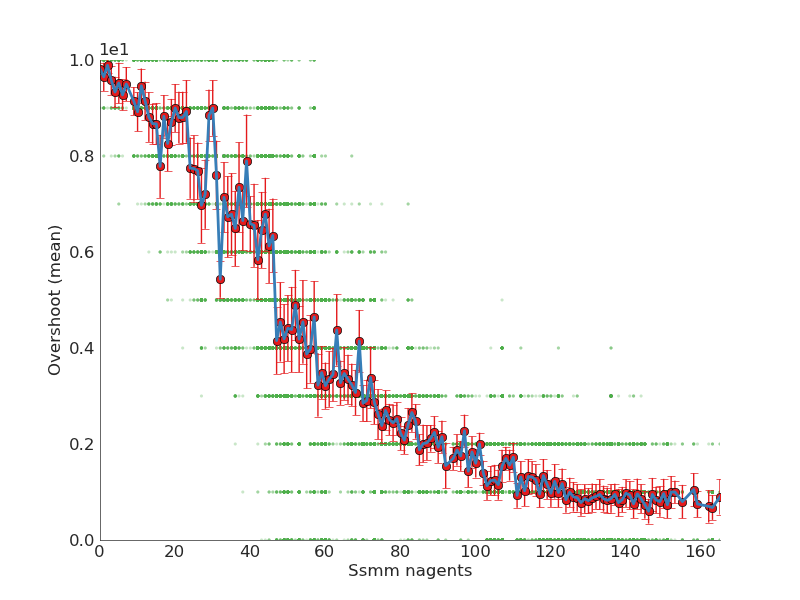
\includegraphics[width=0.5\textwidth]{101_pars_vs_fits/d10/ssmm_nAgents__vs__overshoot(mean)_scatter.png}}
	\subcaptionbox{Correlation between \ssmmnAgents{} and \roundstable\label{fig:d10_parvfit_ssmmnAgents_b}}
	[0.49\linewidth]{\includegraphics[width=0.5\textwidth]{101_pars_vs_fits/d10/ssmm_nAgents__vs__round_stable(mean)_scatter.png}}
	\subcaptionbox{Correlation between \ssmmnAgents{} and \stdev\label{fig:d10_parvfit_ssmmnAgents_c}}
	[0.49\linewidth]{\includegraphics[width=0.5\textwidth]{101_pars_vs_fits/d10/ssmm_nAgents__vs__stdev(mean)_scatter.png}}
	\subcaptionbox{Correlation between \ssmmnAgents{} and \timetoreachnewfundamental\label{fig:d10_parvfit_ssmmnAgents_d}}
	[0.49\linewidth]{\includegraphics[width=0.5\textwidth]{101_pars_vs_fits/d10/ssmm_nAgents__vs__time_to_reach_new_fundamental(mean)_scatter.png}}
	\caption{Correlation between \ssmmnAgents and the four fitness measures in experiment \dten}
	\label{fig:d10_parvfit_ssmmnAgents}
\end{figure}
Figure \ref{fig:d10_parvfit_ssmmnAgents} shows how the number of market makers correlates with the model fitness in experiment \dten. It is clear that a large number of market makers reduces the overshoot, whereas the market virtually always have an overshoot when there are little or no market makers. The same is true for the trade prices flicker: few market makers always means flickering prices. A higher number of market makers makes the market less responsive, while fewer market makers makes the market more responsive. Finally, the number of market makers also influences how quickly the market settles within the stability margin, as markets with more market makers become stable faster than markets with few agents. 

\subsection{Market maker latency}


\subsubsection*{Fixing the number of chartists}
In experiment \dten, the number of chartists was kept fixed at $\scnAgents = 150$, while \ssmmnAgents was varied by the GA. In this case, the \ssmmlatencymu is found to be somewhat correlated with the fitness measures as illustrated on figure \ref{fig:d10_parvfit_ssmmlatencymu}. Especially for $\ssmmlatencymu > 50$, the data seems to be consistent, as the error bars showing the standard deviation of the data are small in this region. However, for $\ssmmlatencymu < 50$, the model behavior is no longer predictable by using \ssmmlatencymu alone. Figure \ref{fig:faster_mm_makes_worse_markets/d10/MM_mmlatency} sheds light on the reason as to why this is, as it shows that even though the market maker latency does influence the market, the effect is secondary to that of the number of agents. For instance, when the market contains less than 25 market makers, all four fitness measures are more or less unchanged shown by the nearly flat red curves. As the number of market makers grow, so does the importance of how fast they are. The average overshoot and the average time to catch up to the new fundamental only change slighly, even with over 100 market makers (yellow line). On the other hand, the average price flickering and the average number of rounds it takes for the market to settle within the stability margin both change significantly with the market maker speed for $\ssmmnAgents > 50$.

\begin{figure}
	%issue 15
	\centering
	\subcaptionbox{Correlation between \ssmmlatencymu and \overshoot\label{fig:d10_parvfit_ssmmlatencymu_a}}
	[0.49\linewidth]{\includegraphics[width=0.5\textwidth]{101_pars_vs_fits/d10/ssmm_latency_mu__vs__overshoot(mean)_scatter.png}}
	\subcaptionbox{Correlation between \ssmmlatencymu and \roundstable\label{fig:d10_parvfit_ssmmlatencymu_b}}
	[0.49\linewidth]{\includegraphics[width=0.5\textwidth]{101_pars_vs_fits/d10/ssmm_latency_mu__vs__round_stable(mean)_scatter.png}}
	\subcaptionbox{Correlation between \ssmmlatencymu and \stdev\label{fig:d10_parvfit_ssmmlatencymu_c}}
	[0.49\linewidth]{\includegraphics[width=0.5\textwidth]{101_pars_vs_fits/d10/ssmm_latency_mu__vs__stdev(mean)_scatter.png}}
	\subcaptionbox{Correlation between \ssmmlatencymu and \timetoreachnewfundamental\label{fig:d10_parvfit_ssmmlatencymu_d}}
	[0.49\linewidth]{\includegraphics[width=0.5\textwidth]{101_pars_vs_fits/d10/ssmm_latency_mu__vs__time_to_reach_new_fundamental(mean)_scatter.png}}
	\caption{Correlation between \ssmmlatencymu{} and fitness values (fixed \scnAgents, variable \ssmmnAgents)}
	\label{fig:d10_parvfit_ssmmlatencymu}
\end{figure}

\begin{comment}
\begin{enumerate}
\item When the market has fast chartists, it needs more market makers to keep the market stable, but these may be slow.
\item When the market has fast chartists, the market first of all needs fast market makers to be stable.
\item A market with few market makers can be stable if the market makers are fast, or if the chartists are slow.
\end{enumerate}
\end{comment}


\begin{figure}
	%issue 15
	\centering
	\subcaptionbox{\label{fig:faster_mm_makes_worse_markets/d10/overshoot_MM_mmlatency}}
	[0.49\linewidth]{\includegraphics[width=0.5\textwidth]{faster_mm_makes_worse_markets/d10/overshoot_MM_mmlatency.png}}
	\subcaptionbox{\label{fig:faster_mm_makes_worse_markets/d10/round_stable_MM_mmlatency}}
	[0.49\linewidth]{\includegraphics[width=0.5\textwidth]{faster_mm_makes_worse_markets/d10/round_stable_MM_mmlatency.png}}
	\subcaptionbox{\label{fig:faster_mm_makes_worse_markets/d10/stdev_MM_mmlatency}}
	[0.49\linewidth]{\includegraphics[width=0.5\textwidth]{faster_mm_makes_worse_markets/d10/stdev_MM_mmlatency.png}}
	\subcaptionbox{\label{fig:faster_mm_makes_worse_markets/d10/time_to_reach_new_fundamental_MM_mmlatency}}
	[0.49\linewidth]{\includegraphics[width=0.5\textwidth]{faster_mm_makes_worse_markets/d10/time_to_reach_new_fundamental_MM_mmlatency.png}}
	\caption{Relation between \ssmmnAgents, \ssmmlatencymu, and the model fitness when the number of chartists was fixed to $\scnAgents = 150 agents$. Due to missing data, some of the curves are not complete.}
	\label{fig:faster_mm_makes_worse_markets/d10/MM_mmlatency}
\end{figure}

In summary, figure \ref{fig:faster_mm_makes_worse_markets/d10/MM_mmlatency} shows that in a market with only a few market makers, these agents have little influence no matter how fast they are. As the number of market makers grow, so does the collective force of all the market makers, and so does the importance of how slow or fast these agents are. The next section will examine how the market behaves with respect to how many chartists are active in the market, and with respect to the latency of the chartists.



\subsubsection{Fixing the number of market makers}XXXNOT FINISHEDXXX
In experiment \deleven, the number of chartists was varied, while the number of market makers were kept at a constant $\ssmmnAgents = 52$ agents. While it was fairly obvious that the market would not be impacted by changing \ssmmlatencymu when only a few market makers were active, it is less obvious that the same is true for the number of chartists. Yet figure 

\begin{figure}
	%issue 15
	\centering
	\subcaptionbox{Correlation between \ssmmlatencymu and \overshoot\label{fig:d11_parvfit_ssmmlatencymu_a}}
	[0.49\linewidth]{\includegraphics[width=0.5\textwidth]{101_pars_vs_fits/d11/ssmm_latency_mu__vs__overshoot(mean)_scatter.png}}
	\subcaptionbox{Correlation between \ssmmlatencymu and \roundstable\label{fig:d11_parvfit_ssmmlatencymu_b}}
	[0.49\linewidth]{\includegraphics[width=0.5\textwidth]{101_pars_vs_fits/d11/ssmm_latency_mu__vs__round_stable(mean)_scatter.png}}
	\subcaptionbox{Correlation between \ssmmlatencymu and \stdev\label{fig:d11_parvfit_ssmmlatencymu_c}}
	[0.49\linewidth]{\includegraphics[width=0.5\textwidth]{101_pars_vs_fits/d11/ssmm_latency_mu__vs__stdev(mean)_scatter.png}}
	\subcaptionbox{Correlation between \ssmmlatencymu and \timetoreachnewfundamental\label{fig:d11_parvfit_ssmmlatencymu_d}}
	[0.49\linewidth]{\includegraphics[width=0.5\textwidth]{101_pars_vs_fits/d11/ssmm_latency_mu__vs__time_to_reach_new_fundamental(mean)_scatter.png}}
	\caption{Correlation between \ssmmlatencymu{} and fitness values (fixed \ssmmnAgents, variable \scnAgents)}
	\label{fig:d11_parvfit_ssmmlatencymu}
\end{figure}


\begin{figure}
     %issue 15
     \centering
     \subcaptionbox{}
     [0.49\linewidth]{\includegraphics[width=0.5\textwidth]{faster_mm_makes_worse_markets/d11/overshoot_SC_mmlatency.png}}
     \subcaptionbox{}
     [0.49\linewidth]{\includegraphics[width=0.5\textwidth]{faster_mm_makes_worse_markets/d11/round_stable_SC_mmlatency.png}}
     \subcaptionbox{}
     [0.49\linewidth]{\includegraphics[width=0.5\textwidth]{faster_mm_makes_worse_markets/d11/stdev_SC_mmlatency.png}}
     \subcaptionbox{}
     [0.49\linewidth]{\includegraphics[width=0.5\textwidth]{faster_mm_makes_worse_markets/d11/time_to_reach_new_fundamental_SC_mmlatency.png}}
     \caption{Relation between \ssmmnAgents, \ssmmlatencymu, and the model fitness when the number of market makers was fixed to $\ssmmnAgents = 52$ agents.}
     \label{fig:faster_mm_makes_worse_markets/d11/SC_mmlatency}
\end{figure}


\subsection{Number of chartists}
\begin{figure}
	%issue 15
	\centering
	\subcaptionbox{Correlation between \scnAgents and \overshoot\label{fig:d11_parvfit_scnagents_a}}
	[0.49\linewidth]{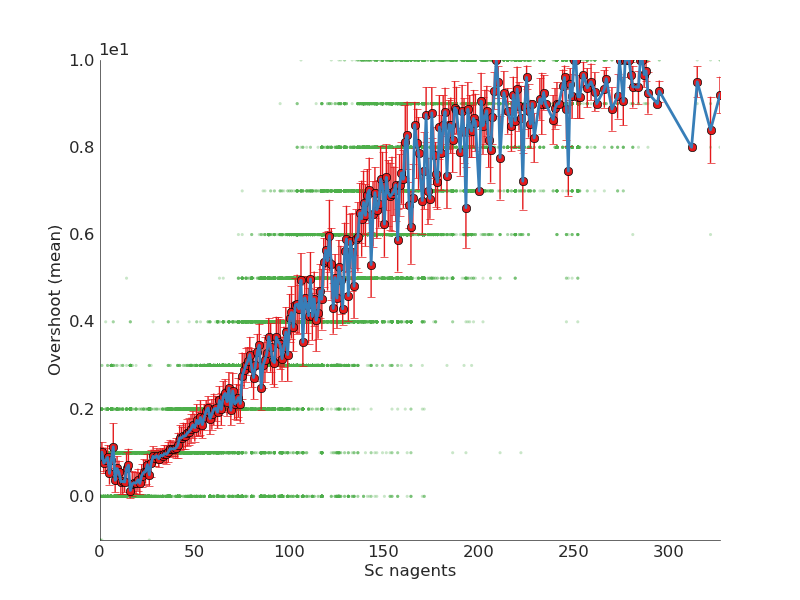
\includegraphics[width=0.5\textwidth]{101_pars_vs_fits/d11/sc_nAgents__vs__overshoot(mean)_scatter.png}}
	\subcaptionbox{Correlation between \scnAgents and \roundstable\label{fig:d11_parvfit_scnagents_b}}
	[0.49\linewidth]{\includegraphics[width=0.5\textwidth]{101_pars_vs_fits/d11/sc_nAgents__vs__round_stable(mean)_scatter.png}}
	\subcaptionbox{Correlation between \scnAgents and \stdev\label{fig:d11_parvfit_scnagents_c}}
	[0.49\linewidth]{\includegraphics[width=0.5\textwidth]{101_pars_vs_fits/d11/sc_nAgents__vs__stdev(mean)_scatter.png}}
	\subcaptionbox{Correlation between \scnAgents and \timetoreachnewfundamental\label{fig:d11_parvfit_scnagents_d}}
	[0.49\linewidth]{\includegraphics[width=0.5\textwidth]{101_pars_vs_fits/d11/sc_nAgents__vs__time_to_reach_new_fundamental(mean)_scatter.png}}
	\caption{Correlation between \scnAgents and the four fitness measures when $\ssmmnAgents = 52$ (experiment \deleven)}
	\label{fig:d11_parvfit_scnagents}
\end{figure}
Figure \ref{fig:d11_parvfit_scnagents} shows the average population wide number of agents $\E{\scnAgents}$ plotted against each of the four fitness measures, and the figures are summarized below.

\begin{itemize}
\item The more chartists a market has, the faster it responds to the fundamental. This is especially true when comparing markets with less than 100 chartists, and less pronounced when comparing markets with over 100 chartists.
\item The model overshoot is also correlated with the number of chartists in such a way that markets with more chartists have a larger overshoot on average. Whereas the market only seemed to benefit from a decreased response time when the number of chartists were kept below 100, the overshoot continues to grow steadily larger even as the number of chartists is increased beyond 100 agents.
\item \stdev is correlated with the number of chartists in the same way as \overshoot, such that more chartists make the traded prices flicker more.
\item Finally, the graph for \roundstable show that the market rarely becomes stable when it contains more than 50 chartists or so.
\end{itemize}
The large errorbars around the points with a large value of \scnAgents is caused by data sparsity in this region. The GA was set to search for stable markets, and since markets with a large number of chartists tend to be unstable, such markets were rarely selected for creating offspring. 





\subsection{Chartist latency}

\subsubsection*{Fixed number of chartists}

Figure \ref{fig:d10_parvfit_sclatencymu_a} shows that \sclatencymu is negatively correlated with \overshoot, such that markets with faster chartists are more likely to have a larger overshoot.  Next, figure \ref{fig:d10_parvfit_sclatencymu}  shows that \sclatencymu is negatively correlated with \stdev, such that markets with faster chartists are more likely to have flickering trade prices. 

As for the market responsiveness, it is seen that \sclatencymu is positively correlated with \timetoreachnewfundamental, such that markets with faster agents is more likely to have a shorter response time to the market. Figure \ref{fig:d10_parvfit_sclatencymu_d} confirms that markets with fast chartists did actually manage to reach the new fundamental price faster than those markets having slow chartists. The average response time of markets in which the chartists had a latency of less than 30 rounds was around 18000 rounds, whereas it was around 25000 rounds with chartists with more than 100 rounds of latency. The market response time is most sensitive in the range $20< \sclatencymu<60$, and does not change much for larger latencies. 

The plots of \overshoot, \stdev and \timetoreachnewfundamental show that predicting the three fitness measures in markets with slow chartists would be more accurate than for markets with fast chartists, as the correlation of \overshoot, \stdev and \timetoreachnewfundamental with \sclatencymu is stronger for larger values of \sclatencymu. 

Figure \ref{fig:d10_parvfit_sclatencymu_b} shows that \sclatencymu is positively correlated with \roundstable, but also that the relationship between \sclatencymu and \roundstable seems highly non-linear. The figure illustrates the binary nature of the stability criteria, that is, that a simulation is either stable or not stable. This causes \roundstable to have a high conditional variance of \roundstable given \sclatencymu in the region $50 < \sclatencymu < 120$, meaning that that prediction of \roundstable from \sclatencymu in this region would not be very accurate. What this means is that the stability of a simulation is highly dependent on factors other than \sclatencymu, when the parameter is within 50 to 120 rounds. When the chartists are faster than 50 rounds, the market is almost always unstable, and when the chartists are slower than 120 rounds the market is almost always stable. 

\begin{figure}
	%issue 15
	\centering
	\subcaptionbox{Correlation between \sclatencymu and \overshoot\label{fig:d10_parvfit_sclatencymu_a}}
	[0.49\linewidth]{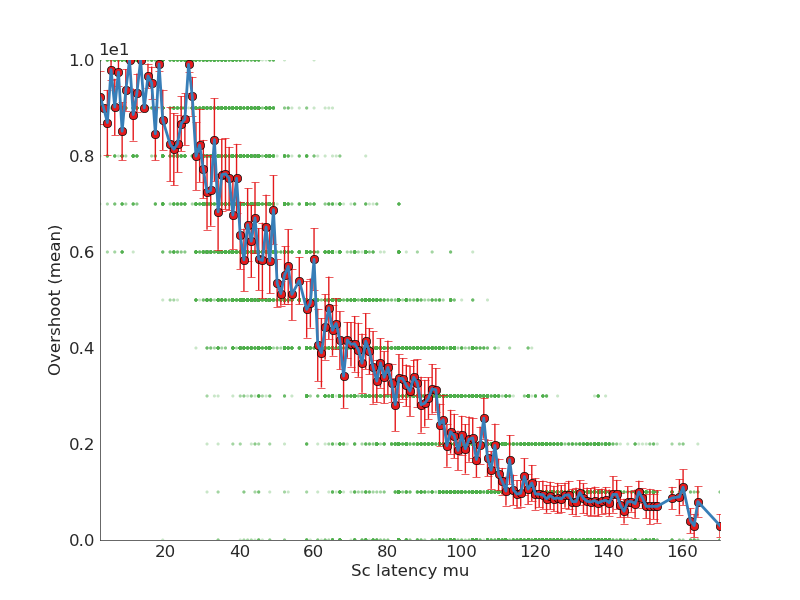
\includegraphics[width=0.5\textwidth]{101_pars_vs_fits/d10/sc_latency_mu__vs__overshoot(mean)_scatter.png}}
	\subcaptionbox{Correlation between \sclatencymu and \roundstable\label{fig:d10_parvfit_sclatencymu_b}}
	[0.49\linewidth]{\includegraphics[width=0.5\textwidth]{101_pars_vs_fits/d10/sc_latency_mu__vs__round_stable(mean)_scatter.png}}
	\subcaptionbox{Correlation between \sclatencymu and \stdev\label{fig:d10_parvfit_sclatencymu_c}}
	[0.49\linewidth]{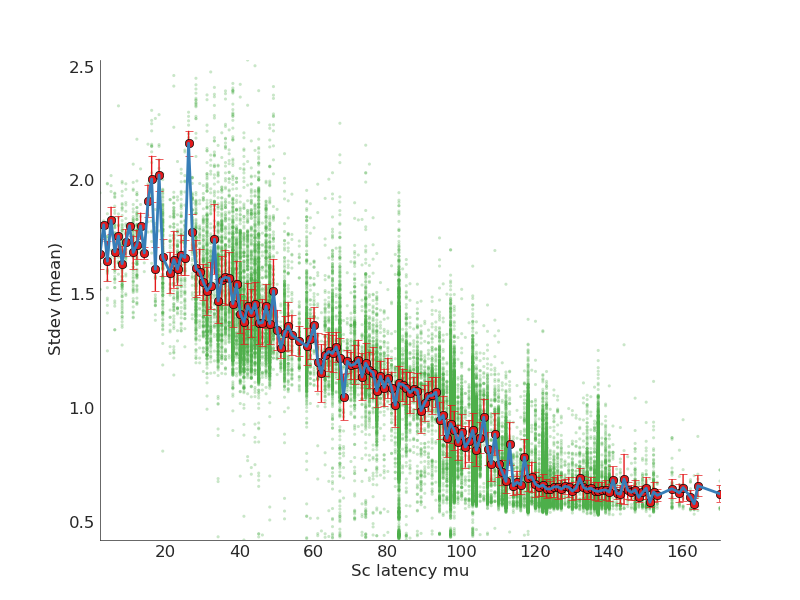
\includegraphics[width=0.5\textwidth]{101_pars_vs_fits/d10/sc_latency_mu__vs__stdev(mean)_scatter.png}}
	\subcaptionbox{Correlation between \sclatencymu and \timetoreachnewfundamental\label{fig:d10_parvfit_sclatencymu_d}}
	[0.49\linewidth]{\includegraphics[width=0.5\textwidth]{101_pars_vs_fits/d10/sc_latency_mu__vs__time_to_reach_new_fundamental(mean)_scatter.png}}
	\caption{Correlation between chartist latency and fitness values (fixed \scnAgents, variable \ssmmnAgents)}
	\label{fig:d10_parvfit_sclatencymu}
\end{figure}

\begin{figure}
	%issue 15
	\centering
	\subcaptionbox{\label{fig:faster_mm_makes_worse_markets/d10/overshoot_MM_sclatency}}
	[0.49\linewidth]{\includegraphics[width=0.5\textwidth]{faster_mm_makes_worse_markets/d10/overshoot_MM_sclatency.png}}
	\subcaptionbox{\label{fig:faster_mm_makes_worse_markets/d10/round_stable_MM_sclatency}}
	[0.49\linewidth]{\includegraphics[width=0.5\textwidth]{faster_mm_makes_worse_markets/d10/round_stable_MM_sclatency.png}}
	\subcaptionbox{\label{fig:faster_mm_makes_worse_markets/d10/stdev_MM_sclatency}}
	[0.49\linewidth]{\includegraphics[width=0.5\textwidth]{faster_mm_makes_worse_markets/d10/stdev_MM_sclatency.png}}
	\subcaptionbox{\label{fig:faster_mm_makes_worse_markets/d10/time_to_reach_new_fundamental_MM_sclatency}}
	[0.49\linewidth]{\includegraphics[width=0.5\textwidth]{faster_mm_makes_worse_markets/d10/time_to_reach_new_fundamental_MM_sclatency.png}}
	\caption{Relation between \ssmmnAgents, \sclatencymu, and the model fitness when the number of chartists was fixed to $\scnAgents = 150 agents$. Due to missing data, some of the curves are not complete.}
	\label{fig:faster_mm_makes_worse_markets/d10/MM_sclatency}
\end{figure}




\subsubsection*{Fixed number of market makers}

\begin{figure}
	%issue 15
	\centering
	\subcaptionbox{Correlation between \sclatencymu and \overshoot\label{fig:d11_parvfit_sclatencymu_a}}
	[0.49\linewidth]{\includegraphics[width=0.5\textwidth]{101_pars_vs_fits/d11/sc_latency_mu__vs__overshoot(mean)_scatter.png}}
	\subcaptionbox{Correlation between \sclatencymu and \roundstable\label{fig:d11_parvfit_sclatencymu_b}}
	[0.49\linewidth]{\includegraphics[width=0.5\textwidth]{101_pars_vs_fits/d11/sc_latency_mu__vs__round_stable(mean)_scatter.png}}
	\subcaptionbox{Correlation between \sclatencymu and \stdev\label{fig:d11_parvfit_sclatencymu_c}}
	[0.49\linewidth]{\includegraphics[width=0.5\textwidth]{101_pars_vs_fits/d11/sc_latency_mu__vs__stdev(mean)_scatter.png}}
	\subcaptionbox{Correlation between \sclatencymu and \timetoreachnewfundamental\label{fig:d11_parvfit_sclatencymu_d}}
	[0.49\linewidth]{\includegraphics[width=0.5\textwidth]{101_pars_vs_fits/d11/sc_latency_mu__vs__time_to_reach_new_fundamental(mean)_scatter.png}}
	\caption{Correlation between chartist latency and fitness values (fixed \ssmmnAgents, variable \scnAgents)}
	\label{fig:d11_parvfit_sclatencymu}
\end{figure}

\begin{figure}
     %issue 15
     \centering
     \subcaptionbox{}
     [0.49\linewidth]{\includegraphics[width=0.5\textwidth]{faster_mm_makes_worse_markets/d11/overshoot_SC_sclatency.png}}
     \subcaptionbox{}
     [0.49\linewidth]{\includegraphics[width=0.5\textwidth]{faster_mm_makes_worse_markets/d11/round_stable_SC_sclatency.png}}
     \subcaptionbox{}
     [0.49\linewidth]{\includegraphics[width=0.5\textwidth]{faster_mm_makes_worse_markets/d11/stdev_SC_sclatency.png}}
     \subcaptionbox{}
     [0.49\linewidth]{\includegraphics[width=0.5\textwidth]{faster_mm_makes_worse_markets/d11/time_to_reach_new_fundamental_SC_sclatency.png}}
     \caption{Relation between \scnAgents, \sclatencymu, and the model fitness when the number of market makers was fixed to $\ssmmnAgents = 52$ agents.}
     \label{fig:faster_mm_makes_worse_markets/d11/SC_sclatency}
\end{figure}

Figures \ref{fig:d11_parvfit_sclatencymu} seems to indicate that no correlations exist between the speed of the chartist agents, and the model fitness measures. However, since figure \ref{fig:d10_parvfit_sclatencymu} does point towards the existence of such correlations, something else must be obscuring the scatter plots in \ref{fig:d11_parvfit_sclatencymu}. The reason is found to be that the number of chartists was not kept constant in experiment \deleven. It turns out that \sclatencymu{} is in fact correlated with \overshoot, \stdev and \timetoreachnewfundamental, but that the correlation depends heavily on the number of chartists in the market. 






\subsection{Chartist to market maker ratio}
\begin{figure}
	%issue 15
	\centering
	\subcaptionbox{}
	[0.49\linewidth]{\includegraphics[width=0.5\textwidth]{101_pars_vs_fits/d10/chartist_per_market_maker__vs__overshoot(mean)_scatter.png}}
	\subcaptionbox{}
	[0.49\linewidth]{\includegraphics[width=0.5\textwidth]{101_pars_vs_fits/d10/chartist_per_market_maker__vs__round_stable(mean)_scatter.png}}
	\subcaptionbox{}
	[0.49\linewidth]{\includegraphics[width=0.5\textwidth]{101_pars_vs_fits/d10/chartist_per_market_maker__vs__stdev(mean)_scatter.png}}
	\subcaptionbox{}
	[0.49\linewidth]{\includegraphics[width=0.5\textwidth]{101_pars_vs_fits/d10/chartist_per_market_maker__vs__time_to_reach_new_fundamental(mean)_scatter.png}}
	\caption{Correlations between \ratioagents and the fitness values when $\scnAgents = 150$}
	\label{fig:parvfit_ratio_d10}
\end{figure}
The above observations about how the number of agents influence the stability and speed of the market pointed out that more market makers made the market slow but stable, while more chartists made the market fast, but unstable. By merging \datamatrixpar{\dten} and \datamatrixpar{\deleven}, we can calculate the ratio, \ratioagents, between the number of chartists and the number of market makers, and see how the fitness values correlate. Figure \ref{fig:parvfit_ratio} shows the resulting scatter plots. 

\begin{figure}
	%issue 15
	\centering
	\subcaptionbox{}
	[0.49\linewidth]{\includegraphics[width=0.5\textwidth]{101_pars_vs_fits/d11/chartist_per_market_maker__vs__overshoot(mean)_scatter.png}}
	\subcaptionbox{}
	[0.49\linewidth]{\includegraphics[width=0.5\textwidth]{101_pars_vs_fits/d11/chartist_per_market_maker__vs__round_stable(mean)_scatter.png}}
	\subcaptionbox{}
	[0.49\linewidth]{\includegraphics[width=0.5\textwidth]{101_pars_vs_fits/d11/chartist_per_market_maker__vs__stdev(mean)_scatter.png}}
	\subcaptionbox{}
	[0.49\linewidth]{\includegraphics[width=0.5\textwidth]{101_pars_vs_fits/d11/chartist_per_market_maker__vs__time_to_reach_new_fundamental(mean)_scatter.png}}
	\caption{Correlations between \ratioagents and the fitness values when $\ssmmnAgents = 52$}
	\label{fig:parvfit_ratio_d11}
\end{figure}








\section{Grouping models by behavior}
This section is be concerned with trying to tie various patterns of model behavior to different regions in the parameter space. The quickest way to get an idea of how the data generated by the simulations is distributed is to make scatter plots. The data of the model fitness is four-dimensional, requiring twelve plots to visualize all combinations. However, since \overshoot is discrete with a small range of values, it is not suitable for a scatter plot. Furthermore, some scatter plots are not useful for interpretation if they do not show any structure in the data. Figure \ref{figure:d9_scatter_fitness} shows three scatter plots which were found to best illustrate the structure of the dataset from \dnine. Note also that coloring each point corresponding to its value in one dimension makes it possible to show how the data is distributed in three dimensions.
\begin{figure}
\centering
\subcaptionbox{$\log \stdev$ vs. $\log \roundstable$ vs. \timetoreachnewfundamental}
[0.49\linewidth]{\includegraphics[width=0.5\textwidth]{21_scatter_plots/d9/d.png}}
\subcaptionbox{\roundstable vs. \timetoreachnewfundamental vs. \stdev}
[0.49\linewidth]{\includegraphics[width=0.5\textwidth]{21_scatter_plots/d9/c.png}}
\subcaptionbox{$\log \overshoot$ vs . $\log \stdev$ vs. \timetoreachnewfundamental}
[0.49\linewidth]{\includegraphics[width=0.5\textwidth]{21_scatter_plots/d9/b.png}}
\caption{Scatter plots of fitness measures in experiment \dnine. }
\label{figure:d9_scatter_fitness}
\end{figure}
The scatter plots do seem to reveal some structure, the presence of large values in the \stdev feature obscures the nature of this structure, in spite of the logarithmic scaling. The plot showing $\log \stdev$ vs. $\log \roundstable$ is squeezed to the left, and the color grading on the scatter plot for $\log \overshoot$ vs . $\log \stdev$ reveals no variety in the \stdev feature. In an attempt to get some more information out of the scatter plot, data points with an overshoot of over 100 \% of the shock to the fundamental (corresponding to $\overshoot > 10$ ) are removed. The resulting scatter plots for the reduced data set are shown on figures \ref{figure:scatter_fitness_inliers_a} and \ref{figure:scatter_fitness_inliers_b}.

First of all, it is seen that while the data is distributed similarly in the three data sets, there are some differences. The data from \dnine{} seems to have many ``lonely'' data points, which are not part of any cluster, whereas the data from \dten{} somehow seems to be the cleanest of the three. In all three data sets, there are clusters of data. The clusters do not necessarily mean anything in themselves. They might simply be due to the way that data points are mutated and crossed by the GA. However, by considering which regions of the fitness space that each cluster covers, it is possible to add meaning to the clusters in terms of model behavior.

\begin{figure}
\centering
\subcaptionbox{Experiment \dnine}[0.49\linewidth]{\includegraphics[width=0.5\textwidth]{103_scatter_manual_outlier/d9/f.png}}
\subcaptionbox{Experiment \dnine}[0.49\linewidth]{\includegraphics[width=0.5\textwidth]{103_scatter_manual_outlier/d9/j.png}}
\subcaptionbox{Experiment \dten}[0.49\linewidth]{\includegraphics[width=0.5\textwidth]{103_scatter_manual_outlier/d10/f.png}}
\subcaptionbox{Experiment \dten}[0.49\linewidth]{\includegraphics[width=0.5\textwidth]{103_scatter_manual_outlier/d10/j.png}}
\subcaptionbox{Experiment \deleven}[0.49\linewidth]{\includegraphics[width=0.5\textwidth]{103_scatter_manual_outlier/d11/f.png}}
\subcaptionbox{Experiment \deleven}[0.49\linewidth]{\includegraphics[width=0.5\textwidth]{103_scatter_manual_outlier/d11/j.png}}
\caption{Scatter plot of \roundstable against \timetoreachnewfundamental with coloring showing $\log \stdev$ and \overshoot}
\label{figure:scatter_fitness_inliers_a}
\end{figure}

\begin{figure}
\centering
\subcaptionbox{Experiment \dnine}[0.49\linewidth]{\includegraphics[width=0.5\textwidth]{103_scatter_manual_outlier/d9/h.png}}
\subcaptionbox{Experiment \dnine}[0.49\linewidth]{\includegraphics[width=0.5\textwidth]{103_scatter_manual_outlier/d9/k.png}}
\subcaptionbox{Experiment \dten}[0.49\linewidth]{\includegraphics[width=0.5\textwidth]{103_scatter_manual_outlier/d10/h.png}}
\subcaptionbox{Experiment \dten}[0.49\linewidth]{\includegraphics[width=0.5\textwidth]{103_scatter_manual_outlier/d10/k.png}}
\subcaptionbox{Experiment \deleven}[0.49\linewidth]{\includegraphics[width=0.5\textwidth]{103_scatter_manual_outlier/d11/h.png}}
\subcaptionbox{Experiment \deleven}[0.49\linewidth]{\includegraphics[width=0.5\textwidth]{103_scatter_manual_outlier/d11/k.png}}
\caption{Scatter plot of $\log \stdev$ against \timetoreachnewfundamental with coloring showing $\roundstable$ and \overshoot}
\label{figure:d9_scatter_fitness_inliers_b}
\end{figure}

\subsection{Manually grouping simulations by behavior}\label{section:manually_grouping_simulations}
Table \ref{table:manual_filtering} contains an overview of the named criteria used for roughly grouping simulations into different types of behavior. The following text contains the reasoning for why each of these groups are interesting.

In figure \ref{figure:scatter_fitness_inliers_a}, the black dashed lines at $\timetoreachnewfundamental = \roundstable$ divide each plot into region A, (upper left triangle) and region B (lower right triangle). Region A contains the fitness-points of the simulations which are counted as stable \textit{after} they reach the new fundamental, and region B contain those that become stable before. 

\subsubsection*{Fast and stable simulations with flickering prices}
The points in the lower left corner in are those which quickly reached the new fundamental price, and quickly because stable, leading those simulations to be assigned low \timetoreachnewfundamental and \roundstable fitness-values. These points are extracted by using filter F1 (see table \ref{table:manual_filtering})

\subsubsection*{Slow or fast and stable simulations with non-flickering prices}
All three data sets have data points which are close to the diagonal. However, only \dnine{} has data points which are close to the diagonal in the upper right corner of the figure. These points are interesting because they belong to simulations which became stable as soon as they reached the new fundamental price. Hence, these simulations should have prices that do not flicker, and therefore yield a small \stdev-fitness. This is confirmed by looking at the left scatter plot of \dnine, as all the points close to the dotted line has a green/blue color. The right plot of \dnine{} shows that these simulations did not have any overshoot. It is interesting that both slow simulations which take a long time to reach the new fundamental, as well as simulations who manage to be fast, have no overshoot, and this observation begs the question of whether or not these simulations have some common parameters that make them behave in such a way. These points are extracted by applying filters F2 and F3 (see table \ref{table:manual_filtering}) to the data matrix \datamatrixfit{\dnine} which selects points that lie within a distance of 400 rounds of the diagonal. 


\subsubsection*{Stable before reaching the new fundamental}
Most of the simulations falling in region B, meaning that they became stable before reaching the new fundamental price, had no overshoot. However, when the model was allowed to have a large number of chartists, but in \deleven, a group of simulations did have a small overshoot. These two groups of points were extracted by applying filters F4 and F5  (see table \ref{table:manual_filtering}).

\subsubsection*{Simulations with overshoot}
XXX NOT FINISHED

\subsubsection{Fast simulations}
All three experiments produces a group of simulations which had a quick response to the shock, but took longer to become stable. The simulations are in the column-shaped cluster in figure \ref{figure:scatter_fitness_inliers_a} and the all have relatively low \timetoreachnewfundamental-fitness of less than 25000 rounds or so. These data points were extracted using filters F7 and F8 (see table \ref{table:manual_filtering}).

\subsubsection*{Unstable simulations with non-flickering prices}
The final group of simulation that are singles out in this section are those that had very smooth price curves (that is, a small value for \stdev), yet did not manage to become stable. These simulations were selected by filter F9.

\begin{figure}
\centering
\subcaptionbox{Experiment \dnine}[0.32\linewidth]{\includegraphics[width=0.32\textwidth]{manual_filtering/d9/group_overlap.png}\label{figure:jaccard_index_a}}
\subcaptionbox{Experiment \dnine}[0.32\linewidth]{\includegraphics[width=0.32\textwidth]{manual_filtering/d10/group_overlap.png}\label{figure:jaccard_index_b}}
\subcaptionbox{Experiment \dten}[0.32\linewidth]{\includegraphics[width=0.32\textwidth]{manual_filtering/d11/group_overlap.png}\label{figure:jaccard_index_c}}
\caption{Jaccard index between the sets of data points extracted by each filter}
\label{figure:jaccard_index}
\end{figure}

The criteria in table \ref{table:manual_filtering} do not prevent a simulation to be selected by different filters. The groups of points are therefore likely to have a non-empty intersection. Using the filters is an the attempt to separate the simulations by their behavior. Hence, the filters should in general not select the same data points. The Jaccard index $J(A,B)$ is calculated between sets $A$ and $B$ and used to determine the overlap between the sets. Figure \ref{figure:jaccard_index} shows the Jaccard index between the sets created by applying the filters to each of the three data sets. Since the distance matrix is symmetrical, only the upper left part has been plotted. In case that the filter produced an empty set, the Jaccard index is undefined, resulting in white squares.

\begin{equation}
J(A,B) = \frac{\lvert A \cap B \rvert}{\lvert A \cup B\rvert }
\end{equation}

\begin{equation}
J(A,B) = \frac{\lvert A \cap B \rvert}{\min \lvert A \rvert, \lvert B\rvert }
\end{equation}


\begin{table}
\centering
\begin{tabular}{l|E|l|E}
\toprule
ID & Target simulations & Filter criteria\\
\midrule
F1 & Fast and stable (but maybe flickering) & $\timetoreachnewfundamental < 12000$, $\roundstable < 12000$, $\log \stdev > 0$ \\
\midrule
F2 & Slow, stable and not flickering (diagonal)& $\lvert \timetoreachnewfundamental - \roundstable \rvert < 400$\\
\midrule 
F3 & Fast and stable and not flickering (diagonal)& $\lvert \timetoreachnewfundamental - \roundstable \rvert < 400$\\
\midrule
F4 & Stable before reaching fundamental, no overshoot& $\roundstable < \timetoreachnewfundamental$, $\overshoot = 0$\\
\midrule
F5 & Stable before reaching fundamental, with overshoot& $\roundstable < \timetoreachnewfundamental$, $\overshoot = >$\\
\midrule
F6 & Has overshoot & $\roundstable > \timetoreachnewfundamental$, $\overshoot > 0$ \\
\midrule
F7 & Fast response, quick to stabilize & $1000 < \timetoreachnewfundamental < 25000$, $20000 < \roundstable < 40000$ \\
\midrule
F8 & Fast response, slow to stabilize & $1000 < \timetoreachnewfundamental < 25000$, $40000 < \roundstable < 75000$ \\
\midrule
F9 & Smooth prices with a small overshoot, yet unstable & $e^{-0.5} - 0.1 < \log \stdev < e^{-0.5} + 0.1$ \\
\midrule
\bottomrule
\end{tabular}
\caption{Filter IDs and fitness-regions}
\label{table:manual_filtering}
\end{table}

\begin{table}
 \centering
 \begin{tabular}{l|rrrrrrrrr}
\toprule
{} &      F1 &      F2 &      F3 &      F4 &      F5 &      F6 &      F7 &      F8 &      F9 \\
\midrule
\sclatencymu                 &    70.1 &    65.5 &    49.5 &    81.5 &    76.7 &    58.5 &    75.8 &    75.6 &    76.0 \\
 \sclatencys                 &     5.4 &     5.5 &     7.8 &     4.5 &     4.9 &     6.8 &     5.0 &     4.9 &     5.0 \\
 \scthinkmu                  &    59.7 &    58.8 &    51.8 &    70.1 &    65.8 &    53.5 &    65.7 &    64.8 &    65.9 \\
 \scthinks                   &    12.0 &    12.0 &    12.8 &    11.2 &    11.6 &    11.2 &    11.4 &    11.6 &    11.6 \\
 \sctimehorizonmu            &  1744.0 &  1676.1 &  1758.1 &  1766.8 &  1773.6 &  1906.9 &  1795.3 &  1757.2 &  1777.9 \\
 \sctimehorizons             &  1483.2 &  1472.7 &  1573.4 &  1415.7 &  1444.2 &  1346.7 &  1437.3 &  1442.4 &  1465.4 \\
 \scwaitTimeBetweenTradingmu &    29.5 &    27.4 &    29.3 &    30.5 &    30.0 &    28.6 &    30.0 &    29.7 &    29.9 \\
 \scwaitTimeBetweenTradings  &     3.2 &     4.1 &     4.2 &     3.0 &     3.1 &     5.1 &     3.1 &     3.0 &     3.1 \\
 \ssmmlatencymu              &    45.2 &    38.5 &    37.6 &    49.8 &    47.3 &    39.2 &    46.1 &    46.3 &    44.5 \\
 \ssmmlatencys               &     4.2 &     4.9 &     4.6 &     4.3 &     4.4 &     5.4 &     4.1 &     4.2 &     5.1 \\
 \ssmmthinkmu                &    39.8 &    38.2 &    40.1 &    37.9 &    38.6 &    35.5 &    39.0 &    39.1 &    35.5 \\
 \ssmmthinks                 &     0.0 &     0.0 &     0.0 &     0.0 &     0.0 &     3.6 &     0.0 &     0.3 &     0.2 \\
 \midrule
\overshoot                   &     1.0 &     1.1 &     1.3 &     0.0 &     1.0 &     3.9 &     1.9 &     2.1 &     1.4 \\
 \roundstable                & 11712.3 & 44993.4 & 13454.5 & 13121.9 & 13468.1 & 80410.6 & 26840.4 & 61259.6 & 54143.9 \\
 \stdev                      &     1.2 &     0.7 &     0.7 &     0.6 &     0.7 &     1.1 &     0.8 &     0.9 &     0.6 \\
 \timetoreachnewfundamental  & 13767.0 & 45089.4 & 13579.4 & 15564.3 & 16743.6 & 16513.3 & 17502.8 & 16812.7 & 40564.2 \\
 \midrule
Count                        &   498 &    33 &  1031 & 33928 & 41982 & 30468 &  2016 &  1733 &  2160 \\
\bottomrule
\end{tabular}
 \label{table:manual_filtering_d9}
 \caption{XXX}
 \end{table}
\begin{table}
 \centering
 \begin{tabular}{l|rrrrrrrrr}
\toprule
{} &      F1 &  F2 &  F3 &      F4 &      F5 &      F6 &      F7 &      F8 &      F9 \\
\midrule
\sclatencymu                &   N/A & N/A & N/A &   123.8 &   121.5 &    78.3 &   116.9 &   104.2 &    95.0 \\
 \sclatencys                &    N/A & N/A & N/A &     6.5 &     6.5 &     9.0 &     7.1 &     8.7 &     8.7 \\
 \ssmmlatencymu             &    N/A & N/A & N/A &    73.9 &    75.8 &    39.2 &    73.3 &    59.6 &    35.9 \\
 \ssmmlatencys              &     N/A & N/A & N/A &     5.6 &     6.0 &     9.6 &     6.6 &     8.7 &     9.2 \\
 \ssmmnAgents               &   N/A & N/A & N/A &   126.5 &   125.6 &    67.1 &   121.2 &    98.0 &    81.2 \\
 \midrule
\overshoot                  &     N/A & N/A & N/A &     0.0 &     1.0 &     4.1 &     1.8 &     2.1 &     0.2 \\
 \roundstable               & N/A & N/A & N/A & 17025.9 & 15920.1 & 81539.2 & 27387.5 & 59444.5 & 24392.3 \\
 \stdev                     &     N/A & N/A & N/A &     0.6 &     0.7 &     1.2 &     0.7 &     0.9 &     0.6 \\
 \timetoreachnewfundamental & N/A & N/A & N/A & 20405.2 & 18724.9 & 15504.3 & 18725.1 & 16840.5 & 31017.6 \\
 \midrule
Count                       &     0 & 0 & 0 &  8486 & 25574 & 47493 &  5379 &  2528 &   399 \\
\bottomrule
\end{tabular}
 \label{table:manual_filtering_d10}
 \caption{XXX}
 \end{table}
\begin{table}
 \centering
 \begin{tabular}{l|rrrrrrrrr}
\toprule
{} &      F1 &  F2 &  F3 &      F4 &      F5 &      F6 &      F7 &      F8 &      F9 \\
\midrule
\sclatencymu                &    N/A & N/A & N/A &    30.4 &    32.3 &    33.3 &    34.3 &    35.1 &    35.8 \\
 \sclatencys                &     N/A & N/A & N/A &     9.3 &     9.9 &     4.6 &     7.2 &     6.6 &     9.0 \\
 \scnAgents                 &    N/A & N/A & N/A &    19.0 &    26.9 &   154.0 &    46.3 &    54.6 &    41.1 \\
 \ssmmlatencymu             &    N/A & N/A & N/A &    67.2 &    55.0 &    38.9 &    50.0 &    47.3 &    46.0 \\
 \ssmmlatencys              &    N/A & N/A & N/A &     8.4 &    11.6 &    22.9 &    17.5 &    19.5 &    14.7 \\
\midrule
\overshoot                  &     N/A & N/A & N/A &     0.0 &     1.0 &    14.6 &     2.0 &     2.6 &     0.0 \\
 \roundstable               & N/A & N/A & N/A & 15678.2 & 15075.3 & 87971.4 & 31954.9 & 63613.9 & 21851.4 \\
 \stdev                     &     N/A & N/A & N/A &     0.7 &     0.8 &     3.6 &     0.9 &     1.0 &     0.6 \\
 \timetoreachnewfundamental & N/A & N/A & N/A & 19965.3 & 18765.4 & 13685.0 & 17265.5 & 16449.5 & 31048.9 \\
 \midrule
Count                       &     0 & 0 & 0 & 71329 & 31377 & 84597 &   349 &  3014 &  1706 \\
\bottomrule
\end{tabular}
 \label{table:manual_filtering_d11}
 \caption{XXX}
 \end{table}
 
Tables \ref{table:manual_filtering_d9}, \ref{table:manual_filtering_d10} and \ref{table:manual_filtering_d11} show the fitness and parameter arithmetic means for each of the nine groups selected by the filters
 
When the number of chartists were fixed as in experiment \dten, the simulations with overshoot (picked out by filter F6) has an average overshot of $\Efilter{6}{\overshoot} = 4.1$ ticks. These markets had comparatively few, but fast market makers ($\Efilter{6}{\ssmmnAgents} = 67.1$ and $\Efilter{6}{\ssmmlatencymu}$), and fast chartists ($\Efilter{6}{\sclatencymu} = 78.3$). Figure \ref{figure:jaccard_index_b} shows that F7 and F8 mostly contain points that are also contained in F6. Both F7 and F8 a lower average overshoot, and this is caused by the markets to have slower chartists, and fewer, slower market makers. When the number of chartists were varied as in experiment \deleven{} (and with a constant of $\ssmmnAgents=52$ market makers), the average latency of the chartists $\Efilter{6}{\sclatencymu}$ did not differ from the other groups. Instead, the biggest difference was that markets with overshoot on average had a high number of chartists. As for the market maker latency, it was smaller than any of the other groups. On the the other hand, markets with no overshoot on average had a large number of marker makers when \scnAgents is fixed to $\scnAgents = 150$, although the market makers were not particularly fast. Markets with no overshoot also had the lowest average number of chartists among the nine groups.


\subsection{Clustering with mixture of Gaussians}
In this section, the focus is shifted from looking at population wide statistics to analysis sub-groups within each population. Whereas the previous sections showed that there do indeed exist statistical relationships between the latency of the agents and the behavior of the model, each discovered correlation was calculated over the entire population. Although the correlations reveal overall tendencies of the model behavior when changing a single parameter, little can be said about how the various parameters interact to determine model behavior. For instance, even though prediction of, say a negative correlation between \timetoreachnewfundamental was \sclatencymu was found, there might be configurations of the model in which faster chartists were actually beneficial to the market. 

One way to approach this problem is to see whether or not there exists relationships between partitions in the parameter space to partitions in the fitness space. As in section \ref{section:filtering_parameters}, the first step is to partition space, since each partition can be interpreted in terms of the model behavior. For instance, a partition covering the lower left half of the 2-dimensional space in figure \ref{figure:scatter_fitness_inliers_a} would encompass all the simulations which had a fast response time and became stable quickly (no matter if they had prices that flickered within the stability margin or not).

In order to investigate this, a Gaussian mixture model (GMM) was used to find clusters in the fitness space. All four fitness measures were used for the clustering. After discarding simulations with undefined fitness values and removing outliers, the data set contained 80813 data points. The large number of data points and the low number of dimensions made it possible to allow a each Gaussian component to have a full covariance matrix, giving the model a high level of flexibility. Figure \ref{fig:d10_scatter_clusters} shows scatter plots of the data after it has been grouped. Tables \ref{table:fit_gmm_all_mean} and \ref{table:fit_gmm_all_std} respectively show the mean and standard deviation calculated over each cluster. The tables are sorted by the average value of \overshoot.



\begin{figure}
	%issue 15
	\centering
	\subcaptionbox{}[0.49\linewidth]{\includegraphics[width=0.5\textwidth]{manually_selected/108_cluster_after_removing_outliers/d10/12_gmm_all_fit_0.png}}
	\subcaptionbox{}[0.49\linewidth]{\includegraphics[width=0.5\textwidth]{manually_selected/108_cluster_after_removing_outliers/d10/12_gmm_all_fit_1.png}}
	\subcaptionbox{}[0.49\linewidth]{\includegraphics[width=0.5\textwidth]{manually_selected/108_cluster_after_removing_outliers/d10/12_gmm_all_fit_2.png}}
	\caption{Scatter plots in fitness space showing the grouping of data points when using a GMM with 12 clusters.}
	\label{fig:d10_scatter_clusters}
\end{figure}

XXX NOT FINISHED. WRITE ABOUT THE CLUSTERS THAT HAVE SOME INTERPRETABLE VALUE. IT DOES NOT HAVE TO BE ALL OF THEM.
$\Varcluster{\roundstable}{8}$ and $\Varcluster{\roundstable}{11}$ and $\Varcluster{\roundstable}{5}$ are large. The points in this cluster have parameters which 



\subsubsection*{Chartist latency and market response time}
As was noted earlier, the evolution of \sclatencymu and \timetoreachnewfundamental indicates that slow chartists made the market slow, and fast chartists made the market fast. C1 is the cluster with the $\Ecluster{\timetoreachnewfundamental}{1}$

\begin{table}
 \centering
 \begin{tabular}{l|rrrr|rrrrr|r}
\toprule
{} &  \overshoot &  \roundstable &  \stdev &  \timetoreachnewfundamental &  \sclatencymu &  \sclatencys &  \ssmmlatencymu &  \ssmmlatencys &  \ssmmnAgents &  \Count \\
\midrule
C1  &         0.0 &       16301.2 &     0.6 &                     19217.4 &         127.2 &          6.2 &            78.4 &            5.2 &         132.2 &  7803 \\
C7  &         0.3 &       24383.1 &     0.7 &                     32005.5 &          87.0 &          9.5 &            25.8 &           10.5 &          66.7 &  1012 \\
C10 &         1.0 &       15832.8 &     0.7 &                     18602.8 &         121.9 &          6.5 &            76.3 &            6.0 &         126.3 & 25245 \\
C8  &         2.0 &       81599.7 &     0.9 &                     16333.6 &         101.8 &          8.7 &            56.4 &            9.2 &          91.3 &  7442 \\
C11 &         2.0 &       30515.0 &     0.7 &                     17822.9 &         114.2 &          7.3 &            71.7 &            7.0 &         117.5 &  5056 \\
C0  &         3.0 &       89015.0 &     1.1 &                     14687.5 &          89.0 &          9.2 &            39.5 &           10.0 &          66.8 &  9201 \\
C5  &         3.0 &       51306.4 &     0.9 &                     16508.7 &         102.2 &          9.0 &            59.2 &            8.8 &          96.0 &   356 \\
C6  &         3.0 &       83914.2 &     1.1 &                     16820.9 &          92.3 &          9.2 &            40.6 &           10.0 &          72.4 &  1598 \\
C9  &         4.0 &       89496.0 &     1.2 &                     14459.8 &          77.7 &          9.6 &            29.9 &           10.4 &          56.7 &  7278 \\
C4  &         5.0 &       89896.6 &     1.4 &                     22034.2 &          62.4 &          9.4 &            21.5 &           10.3 &          51.6 &  5331 \\
C3  &         6.7 &       86440.9 &     1.8 &                     18692.7 &          54.9 &          9.2 &            26.2 &           10.5 &          38.0 &   390 \\
C2  &         7.9 &       89996.1 &     1.6 &                     11574.7 &          36.4 &          9.2 &            26.4 &            9.6 &          36.4 &  10101 \\
Outliers  &        11.5 &       89998.8 &     2.2 &                      8835.1 &          17.8 &          9.3 &            24.3 &            8.5 &          19.4 &   740 \\
\bottomrule
\end{tabular}
 \label{table:d10_gmm_mean}
 \caption{Cluster means (\dten)}
 \end{table}
 
 
 \begin{comment}
 C2 contains the fastest simulations, which take an average of $11.5\times 10^3$ rounds to reach the new fundamental. This group is also the one with the largest overshoot. 
 
 
C7 contains simulations 


Mareket makers are the agents that respond to 


Slow trader match chartist coeincidence
Instead mm match chartists 
If 
Due to the high latency of the slow traders, any order submitted by a slow trader matchng a chartist order i

 \end{comment}

\begin{table}
 \centering
 \begin{tabular}{l|rrrr|rrrrr|r}
\toprule
{} &  \overshoot &  \roundstable &  \stdev &  \timetoreachnewfundamental &  \sclatencymu &  \sclatencys &  \ssmmlatencymu &  \ssmmlatencys &  \ssmmnAgents &  \Count \\
\midrule
C1  &         0.0 &        2142.8 &     0.0 &                      2220.9 &          10.9 &          4.7 &             7.1 &            3.3 &          11.3 &  7803 \\
C7  &         0.5 &        4827.7 &     0.2 &                      7424.7 &          18.4 &          3.8 &            18.7 &            5.4 &          23.2 &  1012 \\
C10 &         0.0 &        2150.8 &     0.1 &                      2261.1 &          12.7 &          4.7 &             9.3 &            4.1 &          14.7 & 25245 \\
C8  &         0.0 &       10563.6 &     0.1 &                      1926.7 &          10.3 &          4.0 &            12.2 &            5.3 &          20.0 &  7442 \\
C11 &         0.0 &        6952.5 &     0.1 &                      2276.1 &          13.8 &          4.7 &            11.6 &            4.7 &          18.3 &  5056 \\
C0  &         0.0 &        1380.7 &     0.1 &                      1479.2 &           9.7 &          3.4 &            14.7 &            5.0 &          12.7 &  9201 \\
C5  &         0.0 &       17151.2 &     0.1 &                      2087.1 &          11.2 &          4.2 &            12.5 &            5.2 &          21.4 &   356 \\
C6  &         0.0 &        3961.3 &     0.1 &                      2646.9 &          10.3 &          3.5 &            16.9 &            5.2 &          16.0 &  1598 \\
C9  &         0.0 &        1048.5 &     0.1 &                      2368.7 &          13.0 &          3.4 &            12.7 &            4.9 &           9.4 &  7278 \\
C4  &         1.4 &         423.6 &     0.2 &                      4246.5 &          21.3 &          4.3 &            11.6 &            5.3 &          10.4 &  5331 \\
C2  &         1.6 &         211.8 &     0.2 &                      1943.0 &          16.0 &          5.2 &            11.7 &            5.5 &          13.7 & 10101 \\
C3  &         2.9 &        7387.0 &     0.4 &                     11884.0 &          26.0 &          4.5 &            15.0 &            5.5 &          30.6 &   390 \\
Outliers  &         0.8 &           0.6 &     0.3 &                      2691.9 &          11.3 &          6.1 &            13.4 &            5.7 &          14.2 &   740 \\
\bottomrule
\end{tabular}
 \label{table:d10_gmm_std}
 \caption{Cluster standard deviations (\dten)}
 \end{table}


\begin{table}
 \centering
 \begin{tabular}{l|rrrr|rrrrr|r}
\toprule
{} &  \overshoot &  \roundstable &  \stdev &  \timetoreachnewfundamental &  \sclatencymu &  \sclatencys &  \scnAgents &  \ssmmlatencymu &  \ssmmlatencys &  \Count \\
\midrule
C5  &         0.0 &       15270.3 &     0.7 &                     19209.4 &          30.0 &          9.3 &        17.5 &            68.7 &            7.9 & 66665 \\
C11 &         0.0 &       21182 &     0.6 &                     29334.9 &          35.5 &          8.9 &        40.2 &            46.6 &           14.5 &  4369 \\
C0  &         1.0 &       14897 &     0.8 &                     18523.0 &          32.2 &         10.0 &        25.9 &            55.6 &           11.3 & 30258 \\
C4  &         1.0 &       19666 &     0.9 &                     25087.1 &          35.3 &          7.3 &        55.5 &            39.0 &           18.9 &  1108 \\
C9  &         1.0 &       30399 &     0.7 &                     35789.7 &          34.4 &          7.8 &        45.6 &            43.6 &           17.9 &   591 \\
C6  &         2.0 &       79198 &     0.9 &                     15620.1 &          37.5 &          6.1 &        63.5 &            47.3 &           20.6 & 11141 \\
C7  &         2.6 &       78771 &     1.0 &                     20524.6 &          37.7 &          5.6 &        63.8 &            38.5 &           22.6 &   967 \\
C1  &         3.0 &       88210 &     1.0 &                     14225.8 &          37.9 &          4.6 &        88.0 &            44.2 &           23.3 & 10577 \\
C8  &         4.0 &       89633 &     1.1 &                     13452.7 &          33.6 &          4.4 &       103.9 &            44.4 &           22.7 &  8099 \\
C3  &         5.7 &       89842 &     1.4 &                     20087.3 &          34.6 &          4.5 &       136.1 &            29.6 &           23.9 &  9613 \\
C10 &         7.0 &       89935 &     1.8 &                     27587.6 &          32.8 &          4.2 &       165.8 &            25.9 &           24.3 &  1401 \\
C2  &         7.0 &       89982 &     1.5 &                     11691.4 &          32.3 &          4.4 &       154.4 &            37.6 &           22.7 & 19067 \\
Outliers  &        40.5 &       89951 &     9.9 &                     10434.7 &          29.2 &          4.0 &       255.5 &            36.4 &           23.5 & 23454 \\
\bottomrule
\end{tabular}
 \label{table:d11_gmm_mean}
 \caption{Cluster means (\deleven)}
 \end{table}
 
 
 \begin{table}
  \centering
  \begin{tabular}{l|rrrr|rrrrr|r}
 \toprule
 {} &  \overshoot &  \roundstable &  \stdev &  \timetoreachnewfundamental &  \sclatencymu &  \sclatencys &  \scnAgents &  \ssmmlatencymu &  \ssmmlatencys &  \Count \\
 \midrule
 C0  &         0.0 &        1349.9 &     0.1 &                      1678.1 &          13.7 &          6.5 &        12.1 &            16.3 &            8.1 & 30258 \\
 C1  &         0.0 &        2448 &     0.1 &                      1383.3 &          16.8 &          4.6 &        15.5 &            18.6 &           10.1 & 10577 \\
 C4  &         0.0 &        3347 &     0.1 &                      4304.5 &          16.8 &          5.7 &        33.3 &            17.4 &           10.8 &  1108 \\
 C5  &         0.0 &        1102 &     0.0 &                      1155.7 &          12.0 &          6.8 &         4.2 &            13.0 &            6.9 & 66665 \\
 C6  &         0.0 &       11795 &     0.1 &                      1640.9 &          17.7 &          5.1 &        18.1 &            19.4 &           10.1 & 11141 \\
 C8  &         0.0 &         893 &     0.1 &                      1446.5 &          16.7 &          4.4 &        19.1 &            20.5 &            9.7 &  8099 \\
 C11 &         0.0 &        2801 &     0.1 &                      4505.8 &          15.0 &          6.4 &        31.7 &            18.6 &           11.2 &  4369 \\
 C7  &         0.6 &        6266 &     0.2 &                      4695.2 &          17.4 &          4.9 &        29.9 &            16.7 &            9.7 &   967 \\
 C9  &         1.1 &        9640 &     0.2 &                     18435.6 &          16.5 &          5.8 &        33.1 &            18.6 &           10.2 &   591 \\
 C2  &         1.7 &         143 &     0.2 &                      1566.7 &          16.3 &          4.7 &        39.8 &            17.6 &            8.9 & 19067 \\
 C3  &         2.2 &         522 &     0.3 &                      3765.1 &          16.7 &          4.5 &        48.7 &            13.0 &            8.9 &  9613 \\
 C10 &         2.3 &         407 &     0.3 &                     10643.3 &          16.8 &          4.4 &        52.4 &            12.4 &            8.8 &  1401 \\

 Outliers  &        53.1 &        1107 &    15.0 &                      3790.6 &          15.5 &          4.5 &        50.7 &            15.9 &            8.3 & 23454 \\
 \bottomrule
 \end{tabular}
  \label{table:d11_gmm_std}
  \caption{Cluster standard deviations (\deleven)}
  \end{table}

 

XXX CONSIDER MOVING SOME OF THE TABLES TO THE APPENDIX?

\section{Summary of results}
XXX NOT FINISHED



